\chapter{Introducción}\label{ch:intro}
\pagenumbering{arabic}
\section{Energía}\label{sec:energy}
La demanda global energética está aumentando en los últimos años principalmente debido al crecimiento demográfico y económico.
El continuo desarrollo de la sociedad moderna requiere que las fuentes de energía sean sostenibles
y respetuosas con el medio ambiente. Sin embargo, hoy en día más del 80\% de la energía mundial proviene
de combustibles fósiles~\cite{/content/publication/caf32f3b-en}, incluyendo carbón, petróleo y gas natural, que están limitados en reserva.
Además, las emisiones de CO$_2$ de este tipo de energía es la principal contribución al aumento del 
efecto invernadero y tiene un efecto importante en el cambio climático. Se
sabe que para nuestro entorno de vida el nivel asequible de aumento de la
temperatura media por encima de los niveles antes de la era industrial es de 2 \centigrade C, más allá del cual es irreversible y casi
se espera que ocurra un cambio climático catastrófico e incontrolable. Este aumento ya ha alcanzado los 0.78 \centigrade C\cite{ip02000c}.
Por lo tanto, es urgente encontrar una manera de reducir la energía relacionada con
los combustibles fósiles. Un alivio a corto plazo sería el desarrollo de nuevas tecnologías para
reducir las emisiones de CO$_2$ de las plantas de energía fósil y mejorar el almacenamiento de CO$_2$ a gran escala,
mientras que una solución a largo plazo debería considerar las alternativas a los combustibles fósiles. Los candidatos con recursos suficientes para hacerse cargo del abastecimiento son la energía solar, la fisión nuclear y
la fusión nuclear~\cite{Freidberg:1186225}.\par
La energía solar es teóricamente amplia e inagotable, pero su intermitencia (luz solo en días sin nubes) y la baja densidad energética (se requiere una gran superficie) hacen difícil construir
una planta de energía solar para producir una cantidad significativa de energía base. La fisión nuclear es
una fuente de energía bien establecida y ha estado produciendo electricidad de carga base durante décadas.
Sin embargo, la eliminación de los residuos nucleares de larga y media vida junto al riesgo de accidente debido a la
reacción en cadena intrínseca de la fisión nuclear ha sido durante mucho tiempo una preocupación pública.\par
La fusión nuclear promete una solución limpia y segura para nuestras necesidades energéticas a largo plazo~\cite{Freidberg:1186225}. 
Primero, las reservas de combustible son abundantes. Para la reacción se necesitan deuterio y tritio, el deuterio puede ser 
extraído del agua de mar; el tritio no se produce de forma natural, pero puede ser obtenido a partir del isótopo de litio $^6$Li. 
Segundo, las reacciones de fusión nuclear no emiten gases de efecto invernadero o cualquier otro daño químico a la atmósfera. 
Tercero, la fusión nuclear es intrínsecamente segura. El combustible de fusión se introduce continuamente en el reactor a una velocidad que sostiene la reacción durante sólo unas pocas decenas
de segundos en cada instante. La reacción de fusión sólo puede ocurrir bajo una temperatura muy alta
y un campo de confinamiento suficientemente preciso y sin reacción en cadena. Cualquier manipulación incorrecta detendrá la reacción.\par
\section{Fusión nuclear}
Los protones y neutrones en el núcleo se mantienen unidos por la fuerza nuclear de corto alcance. La energía
requerida para desmontar un núcleo se llama energía de enlace. La figura~\ref{fig:nucleons} muestra que el promedio
de la energía de enlace varía entre elementos; tanto los núcleos más ligeros como los más pesados tienen un promedio bajo
y los núcleos de masa intermedia tienen la mayor energía de unión.
Esto muestra que la energía nuclear puede obtenerse tanto por la división de núcleos pesados (fisión) como 
fusionando los núcleos ligeros (fusión).\par
\begin{figure}
    \centering
    \def\svgwidth{10cm}
    \input{svg/bindingenergy.pdf_tex}
    \caption[Energía de enlace]{Energía de enlace promedio en función del número másico.}
    \label{fig:nucleons}
\end{figure}
Para lograr una reacción de fusión, dos núcleos necesitan ganar suficiente energía cinética como para superar
la repulsión de Coulomb y alcanzar el régimen de fuerza nuclear de corto alcance. La primera fusión 
se realizó experimentalmente bombardeando sobre un deuterio
objetivo ($^2$H o D) con un rayo de deuterio~\cite{Oliphant1934}, justo después del descubrimiento del deuterio (el isótopo de hidrógeno de masa dos~\cite{PhysRev.40.1}).
Fue durante estos experimentos que el tercer isótopo de hidrógeno, el tritio ($^3$H o T),
se descubrió. Después de este logro, el uso de la fusión nuclear como fuente de energía fue
considerado. Sin embargo, se reconoció que bombardear un objetivo con un chorro acelerado de partículas 
no es factible para la generación de energía, porque la energía utilizada para la aceleración de la partícula
es mucho mayor que la energía producida por la reacción de fusión nuclear y la mayoría de
las partículas aceleradas no daban en el objetivo.\par
\begin{figure}
    \centering
    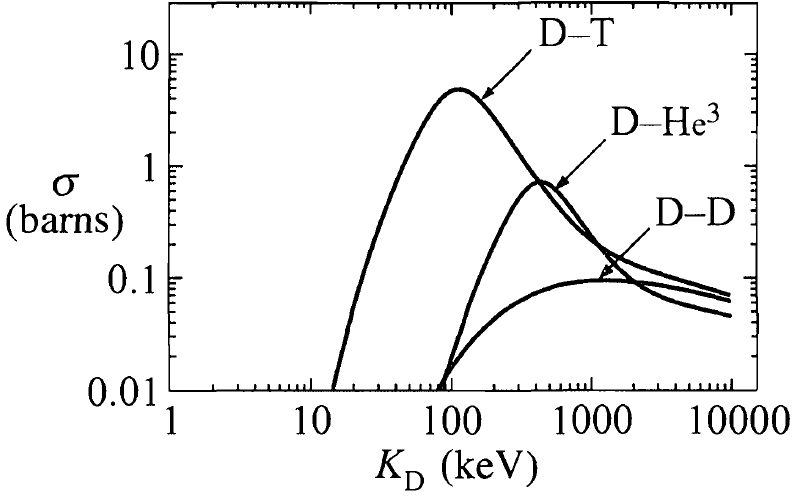
\includegraphics[scale=0.5]{img/fusion.png}
    \caption[Secciones eficaces en reacciones de fusión]{Secciones eficaces para las reacciones de fusión D-T, D-$^3$He y D-D en función de la energía cinética del deuterón K$_D$~\cite{Freidberg:1186225}.}
    \label{fig:fusion}
\end{figure}
Hoy en día se acepta generalmente que la forma más factible para la producción efectiva de energía 
con fusión nuclear es calentar los combustibles de fusión a alta temperatura, para que las partículas se acerquen
con un fuerte movimiento térmico y una reacción nuclear pueda tener lugar. A tan alto nivel de
temperatura, los combustibles de fusión están ionizados y en un estado llamado plasma. La figura~\ref{fig:fusion} muestra las
secciones transversales (probabilidad de que ocurra una reacción nuclear) de diferentes reacciones nucleares.
Podemos ver que la reacción más prometedora es entre el deuterio y el tritio produciendo el neutrón
y una partícula $\alpha$.
\begin{equation}\label{eq:deutreaction}
    D+T\rightarrow\ce{^{4}H}\;(3.5\;MeV)+n\;(14.1\;MeV)
\end{equation}
La energía producida es transportada como energía cinética por el neutrón y la partícula $\alpha$.\par
Uno de los objetivos fundamentales para obtener energía de fusión es mantener la alta temperatura, no con el calentamiento 
externo sino con la energía producida por la reacción nuclear en sí. Este
proceso se llama ignición. Para alcanzar la ignición, el criterio de Lawson~\cite{Lawson_1957} predice que 
debe cumplirse la siguiente condición:
\begin{equation}\label{eq:lawson}
    nT\tau_e\geq3\times10^{21}\:keVs/m^{3}
\end{equation}
donde n es la densidad del plasma, T es la temperatura y $\tau_e$ es el tiempo de confinamiento produciendo energía.
Este triple producto sugiere que para generar energía de forma efectiva a partir de la fusión nuclear, el plasma
necesita estar confinado a muy alta temperatura por un tiempo suficientemente largo con alta densidad.
Hay principalmente dos formas de conseguir energía de fusión controlada: el confinamiento magnético 
y el confinamiento inercial. En este trabajo se centra en la primera de ellas.\par
